\section{Introduction}

The generation of high-quality educational explanations represents a fundamental challenge in natural language processing. Unlike general-purpose conversational tasks, educational rationales must adhere to strict logical constraints, factual accuracy, and pedagogical clarity. While Supervised Fine-Tuning (SFT) has enabled Large Language Models (LLMs) to produce highly fluent responses, these models frequently suffer from two critical deficiencies: hallucination of facts and "verbosity bias"---the tendency to generate excessively long, rhetorical text to mask underlying logical inconsistencies.

Recent advancements in alignment engineering, such as Proximal Policy Optimization (PPO) and Direct Preference Optimization (DPO), have sought to optimize models to adhere to human preferences. However, these techniques largely rely on reward models trained on stylistic human preferences, which inadvertently reward verbose, "helpful-sounding" but factually shallow rhetoric. Furthermore, when researchers attempt to optimize strictly for deterministic logical metrics, such as Natural Language Inference (NLI) entailment, they often encounter what we define as the \textbf{"alignment tax"}---a phenomenon where the model's linguistic fluency and grammatical coherence collapse in favor of robotic, repetitive, yet logically sound snippets.

\begin{figure}[h]
\centering
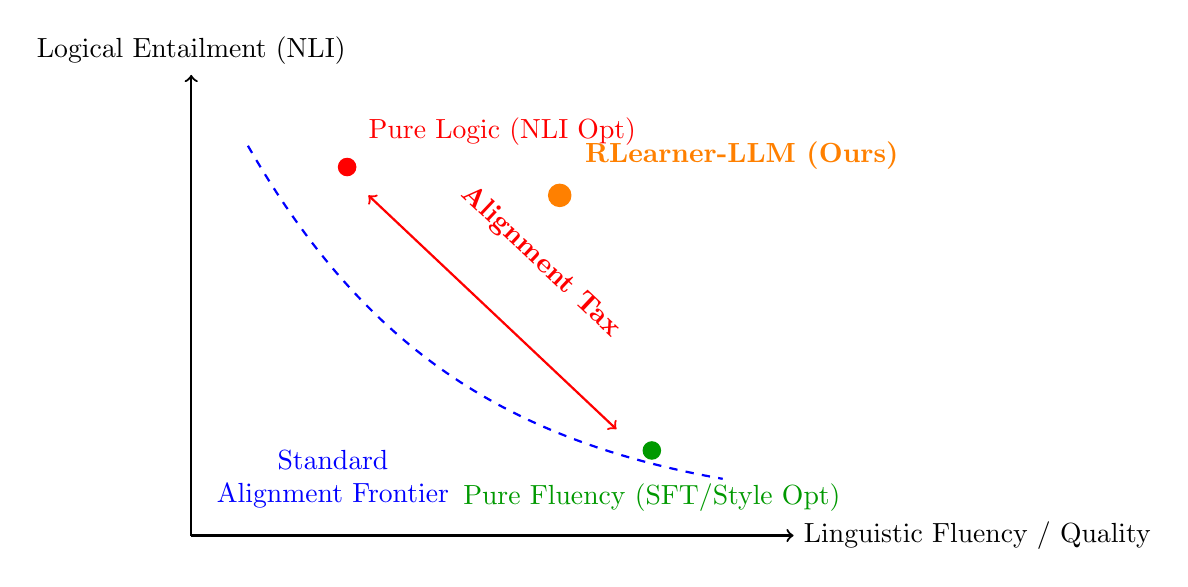
\begin{tikzpicture}[scale=0.9]
% Axes
\draw[->, thick] (0,0) -- (8.5,0) node[right] {Linguistic Fluency / Quality};
\draw[->, thick] (0,0) -- (0,6.5) node[above] {Logical Entailment (NLI)};

% Curves
\draw[blue, thick, dashed] (0.8,5.5) to[bend right=25] (7.5,0.8);
\node[blue, align=center] at (2.0,0.8) {Standard\\Alignment Frontier};

% Points - Moved right as requested
\filldraw[red] (2.2,5.2) circle (3.5pt) node[above right=0.15cm] {Pure Logic (NLI Opt)};
\filldraw[green!60!black] (6.5,1.2) circle (3.5pt) node[below=0.3cm] {Pure Fluency (SFT/Style Opt)};
\filldraw[orange] (5.2,4.8) circle (4.5pt) node[above right=0.2cm, orange] {\textbf{RLearner-LLM (Ours)}};

% Annotations - Separated from the dots
\draw[<->, red, thick] (2.5,4.8) -- (6.0,1.5) node[midway, sloped, above=0.6cm] {\textbf{Alignment Tax}};

\end{tikzpicture}
\caption{Conceptual illustration of the \textbf{Alignment Tax}. Standard optimization techniques often force a trade-off between logical grounding and linguistic fluency. RLearner-LLM aims to push the boundary toward the upper-right quadrant.}
\label{fig:alignment_tax}
\end{figure}

In this paper, we propose \textbf{RLearner-LLM} (utilizing Hybrid-DPO), a cross-domain alignment framework designed to eliminate this tax. By fusing deterministic logical entailment signals from NLI models with holistic fluency scores from a secondary verifier model, RLearner-LLM curates high-fidelity pairwise preference data without the need for expensive human-in-the-loop intervention. This dual-reward signal ensures that the model learns to prioritize factual grounding while maintaining the linguistic naturalness required for effective pedagogy.

Our contributions are summarized as follows:
\begin{enumerate}
    \item We demonstrate the severe limitations of current LLM-as-a-judge evaluation paradigms, highlighting a systematic self-preference verbosity bias that penalizes concise, logical explanations.
    \item We introduce the \textbf{RLearner-LLM} framework, an automated pipeline for generating preference pairs ($\mathcal{D}_{pref}$) that balance factual density with stylistic coherence.
    \item We provide an empirical validation across five distinct academic domains (Biology, Medicine, Law), demonstrating that \textbf{RLearner-LLM} achieves up to a 5$\times$ improvement in logical entailment scores over SFT baselines while maintaining high user win rates in side-by-side evaluations.
\end{enumerate}
